\documentclass[10pt,letterpaper]{article}
\usepackage[margin=0.75in]{geometry}
\usepackage{graphicx}
\usepackage{booktabs}
\usepackage{enumitem}
\usepackage{hyperref}
\usepackage{xcolor}
\usepackage{amsmath}
\usepackage{tikz}
\usetikzlibrary{shapes,arrows,positioning,fit,backgrounds}
\usepackage{titlesec}
\titlespacing*{\section}{0pt}{8pt}{4pt}
\titlespacing*{\subsection}{0pt}{6pt}{3pt}
\setlength{\parskip}{2pt}

\title{\textbf{Adaptive RDMA Optimization for Distributed LLM Workloads}\\[0.5em]
\large Implementation Plan}
\author{Nathan Gopee\\
MS Computer Science, SUNY New Paltz\\
\texttt{gopeen1@newpaltz.edu}\\[1em]
\small Advisors: Dr. Wafi Danesh \& Dr. Ashley Suchy}
\date{January 2026}

\begin{document}
\maketitle

\section{Problem Statement}

Distributed large language model inference suffers from communication bottlenecks that manifest as Time-To-First-Token (TTFT) latency. Current systems like vLLM use NCCL for GPU-to-GPU communication, which employs static routing strategies optimized for bulk transfers. This creates \textbf{head-of-line blocking}: small, latency-sensitive tensors (KV cache pages, attention scores) wait behind large bulk transfers (model weights, gradient accumulations).

This thesis develops an \textbf{adaptive RDMA middleware} that classifies tensor access patterns at runtime and routes transfers through dedicated paths---low-latency channels for frequently-accessed ``hot'' data and throughput-optimized channels for ``cold'' bulk transfers.

\section{What vLLM Already Provides}

Before defining contributions, it is essential to understand vLLM's existing architecture:

\begin{table}[h]
\centering
\small
\begin{tabular}{@{}ll@{}}
\toprule
\textbf{Feature} & \textbf{vLLM Implementation} \\
\midrule
KV Cache Management & PagedAttention with block-based allocation \\
Request Scheduling & Continuous batching with FCFS/priority policies \\
Single-Node Multi-GPU & \texttt{MultiProcExecutor} with tensor parallelism \\
Multi-Node Distribution & Ray + pipeline parallelism \\
GPU Communication & NCCL (all-reduce, all-gather) \\
KV Transfer (Disagg. P/D) & NIXL-based connectors (LMCache, NixlConnector) \\
Disaggregated Serving & Prefill/decode separation via llm-d orchestrator \\
External KV Cache & LMCacheConnectorV1 for vLLM V1 integration \\
Optimizations & Chunked prefill, prefix caching, speculative decoding \\
\bottomrule
\end{tabular}
\caption{vLLM capabilities this work builds upon, not replaces.}
\end{table}

vLLM's distributed execution uses \texttt{MultiProcExecutor}, which spawns worker processes coordinated via shared-memory message queues. Inter-GPU communication occurs through NCCL, which discovers network topology at initialization but does not adapt routing based on runtime access patterns.

\subsection{Recent vLLM Ecosystem Developments (2025--2026)}

Since the initial proposal, significant advancements have emerged in the vLLM ecosystem:

\textbf{vLLM v0.15.0} (Current): PyTorch 2.9.0 with CUDA 12.9, Model Runner V2 (experimental), improved distributed inference with DP+MoE fixes.

\textbf{NIXL} (NVIDIA Dynamo): Communication abstraction layer supporting NVLink, RDMA-capable NICs, and GPU Direct Storage. Enables high-bandwidth KV cache transfer between disaggregated prefill and decode instances.

\textbf{llm-d} (v0.4, Dec 2025): Disaggregated serving orchestrator achieving 40\% reduction in per-output-token latency on DeepSeek V3.1. Supports RDMA over RoCE for point-to-point KV cache transfer via NIXL sidecar.

\textbf{LMCache}: External KV cache layer for vLLM V1 with first-class NIXL support. Enables KV cache extraction/injection directly from vLLM's internal paged memory.

\textbf{Semantic Router v0.1 Iris} (Jan 2026): Intelligent model routing layer with signal-decision architecture, modular LoRA optimization, and HaluGate safety pipeline.

\section{Thesis Contribution}

This work introduces three components that integrate with vLLM's existing infrastructure:

\subsection{Unified Telemetry Layer}
A monitoring system that instruments tensor transfers to collect:
\begin{itemize}[noitemsep]
    \item Access frequency per tensor/KV block
    \item Transfer size distributions
    \item Queue depth at RDMA endpoints
    \item Latency percentiles (p50, p95, p99)
\end{itemize}

\subsection{WFA-Based Adaptive Classifier}
A Weighted Finite Automaton that classifies tensors into hot/cold categories based on observed patterns. States transition based on access frequency:

\begin{center}
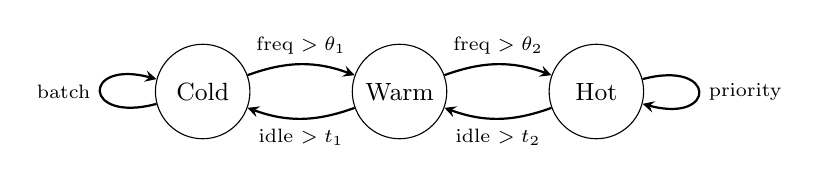
\begin{tikzpicture}[node distance=2.5cm, auto,
    state/.style={circle, draw, minimum size=1.2cm, font=\small},
    arrow/.style={->, >=stealth, thick}]

    \node[state] (cold) {Cold};
    \node[state, right of=cold] (warm) {Warm};
    \node[state, right of=warm] (hot) {Hot};

    \draw[arrow, bend left=20] (cold) to node[above] {\scriptsize freq $> \theta_1$} (warm);
    \draw[arrow, bend left=20] (warm) to node[below] {\scriptsize idle $> t_1$} (cold);
    \draw[arrow, bend left=20] (warm) to node[above] {\scriptsize freq $> \theta_2$} (hot);
    \draw[arrow, bend left=20] (hot) to node[below] {\scriptsize idle $> t_2$} (warm);

    \draw[arrow, loop left] (cold) to node[left] {\scriptsize batch} (cold);
    \draw[arrow, loop right] (hot) to node[right] {\scriptsize priority} (hot);
\end{tikzpicture}
\end{center}

The classifier also detects workload phase (prefill vs.\ decode, training vs.\ inference) to adjust thresholds dynamically.

\subsection{Smart RDMA Routing Layer}
Dual-path routing implemented via \texttt{pyverbs} (libibverbs Python bindings):

\begin{itemize}[noitemsep]
    \item \textbf{Hot Path}: Dedicated Queue Pairs (QPs) with polled completions, RDMA Write with Immediate for sub-5$\mu$s transfers
    \item \textbf{Cold Path}: Batched transfers with event-driven completions, optimized for throughput over latency
\end{itemize}

Memory registration uses NUMA-aware allocation via \texttt{libnuma}:
\begin{itemize}[noitemsep]
    \item \texttt{numa\_bind\_to\_node()}: Pin RDMA buffers to the same NUMA node as the HCA, avoiding QPI/UPI traversal penalties (40\%+ throughput loss)
    \item \texttt{numa\_interleave\_nodes()}: For large tensors spanning multiple nodes, interleave allocation across NUMA domains
    \item Automatic NUMA topology detection via \texttt{/sys/devices/system/node/}
\end{itemize}

\subsection{Transport Layer Options}

The middleware supports multiple transport backends with different performance characteristics:

\begin{table}[h]
\centering
\small
\begin{tabular}{@{}lccc@{}}
\toprule
\textbf{Transport} & \textbf{Latency} & \textbf{Infrastructure} & \textbf{GPU Support} \\
\midrule
SoftRoCE & $\sim$10$\mu$s & Standard Ethernet & All GPUs \\
Tesla TTPoe & $\sim$1--2$\mu$s & Commodity switches & All GPUs \\
RoCEv2 & $\sim$4--5$\mu$s & DCB/PFC switches & All GPUs \\
InfiniBand & $\sim$2--3$\mu$s & IB fabric & All GPUs \\
GPUDirect RDMA & $<$2$\mu$s & RoCE/IB + nvidia-peermem & Tesla/Quadro only \\
\bottomrule
\end{tabular}
\caption{Transport layer comparison for distributed inference.}
\end{table}

\textbf{Tesla TTPoe}: A peer-to-peer Ethernet transport designed for exascale AI (Tesla Dojo). Unlike RoCE/InfiniBand which require lossless fabrics, TTPoe is a \textit{lossy} protocol that expects packet loss and handles retries locally. This eliminates Priority Flow Control (PFC) requirements and works on commodity switches. Reference implementation available as Linux kernel module.

\textbf{GPUDirect RDMA}: Enables NICs to read/write GPU memory directly without CPU involvement. Requires \texttt{nvidia-peermem} kernel module and GPU/NIC on same PCIe root complex. \textit{Critical limitation}: Only supported on datacenter GPUs (Tesla, Quadro); consumer GPUs (GeForce RTX) lack the necessary BAR mapping features.

\textbf{NIXL}: NVIDIA's communication abstraction from Dynamo, providing unified API across NVLink, RDMA, and TCP. Used by LMCache and llm-d for disaggregated KV cache transfer.

\section{Architecture}

\begin{figure}[h]
\centering
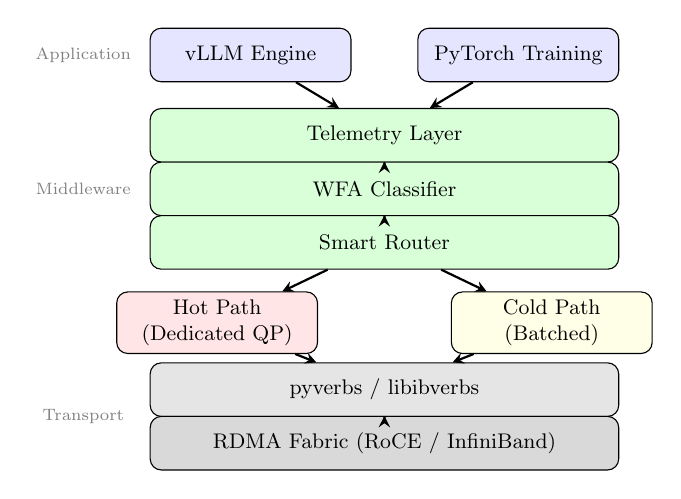
\begin{tikzpicture}[
    scale=0.85, transform shape,
    box/.style={rectangle, draw, rounded corners, minimum width=3cm, minimum height=0.8cm, align=center, font=\small},
    widebox/.style={rectangle, draw, rounded corners, minimum width=7cm, minimum height=0.8cm, align=center, font=\small},
    arrow/.style={->, >=stealth, thick}
]

% Application Layer
\node[box, fill=blue!10] (vllm) at (0,4) {vLLM Engine};
\node[box, fill=blue!10] (pytorch) at (4,4) {PyTorch Training};

% Middleware Layer
\node[widebox, fill=green!15] (telem) at (2,2.8) {Telemetry Layer};
\node[widebox, fill=green!15] (wfa) at (2,2) {WFA Classifier};
\node[widebox, fill=green!15] (router) at (2,1.2) {Smart Router};

% Split paths
\node[box, fill=red!10] (hot) at (-0.5,0) {Hot Path\\(Dedicated QP)};
\node[box, fill=yellow!10] (cold) at (4.5,0) {Cold Path\\(Batched)};

% RDMA Layer
\node[widebox, fill=gray!20] (pyverbs) at (2,-1) {pyverbs / libibverbs};
\node[widebox, fill=gray!30] (rdma) at (2,-1.8) {RDMA Fabric (RoCE / InfiniBand)};

% Arrows
\draw[arrow] (vllm) -- (telem);
\draw[arrow] (pytorch) -- (telem);
\draw[arrow] (telem) -- (wfa);
\draw[arrow] (wfa) -- (router);
\draw[arrow] (router) -- (hot);
\draw[arrow] (router) -- (cold);
\draw[arrow] (hot) -- (pyverbs);
\draw[arrow] (cold) -- (pyverbs);
\draw[arrow] (pyverbs) -- (rdma);

% Labels
\node[font=\scriptsize, gray] at (-2.5, 4) {Application};
\node[font=\scriptsize, gray] at (-2.5, 2) {Middleware};
\node[font=\scriptsize, gray] at (-2.5, -1.4) {Transport};

\end{tikzpicture}
\caption{System architecture showing middleware integration points.}
\end{figure}

\subsection{Integration Points}

The middleware intercepts communication at two levels:

\textbf{1. Tensor Parallel Communication} (replacing NCCL): The adaptive middleware hooks into vLLM's tensor-parallel all-reduce path (in \texttt{vllm/distributed/parallel\_state.py}). When a tensor all-reduce is requested, the WFA classifier first determines whether the tensor exhibits hot or cold access patterns. Hot tensors are routed through a dedicated low-latency RDMA channel, while cold tensors are batched and sent through the throughput-optimized channel. This replaces the default \texttt{torch.distributed.all\_reduce} call with pattern-aware routing.

\textbf{2. KV Cache Transfers} (extending vLLM's Connector abstraction): A new \texttt{AdaptiveRDMAConnector} class extends vLLM's \texttt{KVConnectorBase}. During KV layer save operations, each KV block is classified by the WFA classifier and then routed through the appropriate RDMA transfer path based on its access pattern.

\section{Implementation Plan}

\subsection{Phase 1: Foundation}

\textbf{Environment Setup:} The RDMA software stack (\texttt{rdma-core}, \texttt{ibverbs-utils}, \texttt{perftest}, \texttt{libibverbs-dev}, and \texttt{pyverbs}) is installed on both nodes. Soft-RoCE is enabled on the 10GbE interface by loading the \texttt{rdma\_rxe} kernel module and creating a virtual RDMA device. Connectivity is verified using \texttt{ibv\_devices} to list RDMA devices and \texttt{rping} for basic RDMA ping testing between server and client.

\textbf{Baseline Latency Measurement:} RDMA write latency is measured using \texttt{ib\_write\_lat} from the perftest suite, targeting sub-10$\mu$s round-trip time on Soft-RoCE. TCP latency is measured with \texttt{sockperf} to establish a baseline for comparison against RDMA performance.

\textbf{pyverbs Buffer Pool Implementation:} A NUMA-aware RDMA buffer pool is implemented using \texttt{pyverbs}. The pool allocates a large memory region (default 256MB) registered with the RDMA protection domain, pinned to the same NUMA node as the host channel adapter using \texttt{libnuma}. A sub-allocation strategy provides individual buffers from this registered region on demand, avoiding repeated memory registration overhead.

\textbf{Deliverable}: RDMA ping-pong achieving $<$10$\mu$s RTT on SoftRoCE.

\subsection{Phase 2: Telemetry \& Classification}

\textbf{Instrument vLLM's KV Cache Manager:} An instrumented subclass of vLLM's \texttt{KVCacheManager} is created that logs access timestamps for every block allocation. Each call to \texttt{allocate\_slots} records a nanosecond-precision timestamp per block, building an access frequency histogram that feeds into the classifier.

\textbf{Implement WFA Classifier:} The \texttt{TensorClassifier} maintains a state machine with three states (Cold, Warm, Hot) for each tracked tensor. Transitions are governed by configurable thresholds: tensors exceeding $\theta_1$ accesses per interval transition from Cold to Warm, and those exceeding $\theta_2$ transition from Warm to Hot. Idle periods longer than $t_{idle}$ cause demotion. The classifier tracks per-tensor state and last-access timestamps to make classification decisions.

\textbf{Phase Detection (Prefill vs Decode):} A lightweight heuristic distinguishes prefill from decode phases by examining the ratio of tokens to sequences in each batch. Prefill phases exhibit many tokens across few sequences, while decode phases show one token per sequence across many sequences. A threshold of eight tokens per sequence separates the two regimes, allowing the classifier to adjust its routing thresholds accordingly.

\textbf{Deliverable}: Classifier tested on synthetic access patterns with accuracy reported.

\subsection{Phase 3: Routing Integration}

\textbf{Dual-Path Queue Pair Pool:} The \texttt{DualPathRDMA} class maintains separate pools of RDMA Queue Pairs for hot and cold traffic. Hot-path QPs (default: 4) use polled completions for minimal latency, executing RDMA Write with Immediate operations targeting sub-5$\mu$s transfer times. Cold-path QPs (default: 2) use event-driven completions and batch transfers---accumulating tensors until a batch threshold (default: 8) is reached before flushing, optimizing for throughput. A least-loaded selection policy distributes hot transfers across available QPs.

\textbf{vLLM Connector Integration:} A new \texttt{AdaptiveRDMAConnector} (placed in \texttt{vllm/distributed/kv\_transfer/}) extends \texttt{KVConnectorBase} and wires together the \texttt{DualPathRDMA} transport with the \texttt{TensorClassifier}. During \texttt{save\_kv\_layer} operations, each block's access count and time since last access are fed to the classifier, and the resulting classification determines which RDMA path handles the transfer.

\textbf{Benchmark TTFT Improvement:} The vLLM OpenAI-compatible API server is launched with the adaptive connector enabled (via the \texttt{--kv-connector AdaptiveRDMAConnector} flag) using tensor parallelism across two GPUs. TTFT is measured using vLLM's built-in benchmark serving script across 100 prompts.

\textbf{Deliverable}: Measured TTFT comparison between adaptive RDMA and NCCL baseline on 7B model inference.

\subsection{Phase 4: Training Extension}

\textbf{Adaptive All-Reduce for Gradients:} An \texttt{AdaptiveAllReduce} class hooks into PyTorch DDP gradient synchronization. Gradient tensors are classified based on magnitude variance---critical gradients with high variance are synchronized immediately via the hot RDMA path, while bulk gradients with stable values are batched and synchronized asynchronously through the cold path.

\textbf{Integration with FSDP:} The adaptive routing is integrated with PyTorch's Fully Sharded Data Parallel (FSDP) by wrapping the model with an \texttt{AdaptiveProcessGroup} that routes FSDP's internal communication through the dual-path RDMA infrastructure.

\textbf{Profiling:} NVIDIA Nsight Systems is used to profile training runs with adaptive RDMA enabled, generating detailed timelines of communication overlap and identifying any remaining synchronization bottlenecks.

\textbf{Deliverable}: Measured training throughput comparison between adaptive RDMA and NCCL baseline.

\subsection{Phase 5: Validation \& Writing}

\textbf{Comprehensive Benchmarking:} A full sweep of model sizes (7B, 13B, 70B parameters) and tensor-parallel configurations (2, 4, 8 GPUs) is executed, comparing NCCL baseline against the adaptive RDMA connector. Metrics collected include TTFT, time per output token, and aggregate throughput.

\textbf{Ablation Studies:}
\begin{itemize}[noitemsep]
    \item WFA classifier vs.\ static hot/cold assignment
    \item Hot-path only vs.\ dual-path routing
    \item NUMA-aware vs.\ NUMA-oblivious allocation
    \item Threshold sensitivity analysis ($\theta_1$, $\theta_2$, $t_{idle}$)
\end{itemize}

\textbf{Deliverable}: Complete thesis with reproducible benchmarks and defense.

\section{Evaluation Plan}

The following metrics will be measured to evaluate the adaptive RDMA middleware against the NCCL baseline. Baseline and target values will be determined experimentally:

\begin{table}[h]
\centering
\small
\begin{tabular}{@{}llll@{}}
\toprule
\textbf{Metric} & \textbf{Baseline} & \textbf{Target} & \textbf{Measurement} \\
\midrule
TTFT (7B model) & Measured via NCCL & Reduce vs baseline & vLLM benchmark suite \\
TTFT (multi-node) & Measured via NCCL & Reduce vs baseline & vLLM benchmark suite \\
P99 latency variance & Measured (HOL present) & Reduce variance & Custom telemetry \\
Gradient sync overhead & Measured via profiler & Reduce vs baseline & PyTorch profiler \\
\bottomrule
\end{tabular}
\caption{Evaluation metrics---baselines and improvements to be determined experimentally.}
\end{table}

\section{Hardware \& Software Requirements}

\textbf{Lab Hardware (SUNY New Paltz)}:
\begin{itemize}[noitemsep]
    \item Cerberus: 2$\times$ RTX 5090 (32GB each)
    \item Chimera: 3$\times$ RTX 3090 (24GB each)
    \item Network: 10GbE with SoftRoCE, potential 100GbE upgrade
\end{itemize}

\textbf{Home Lab Hardware}:
\begin{itemize}[noitemsep]
    \item Tower 1 (Windows): Ryzen 9 7950X, 192GB DDR5, RTX 5070 Ti (16GB GDDR7)
    \item Tower 2 (Proxmox): Xeon E5-2697A v4, 128GB DDR4, 2$\times$ Tesla V100 32GB
    \item Network: 100GbE Mellanox ConnectX-4 with SoftRoCE (already deployed)
    \item Total: 32 cores, 320GB RAM, 80GB VRAM
\end{itemize}

\textit{Note: The V100s and RTX 5090s support GPUDirect RDMA; the RTX 5070 Ti and RTX 3090s do not (consumer GPUs lack this feature). Home lab has 100GbE networking ready for RDMA testing; lab upgrade pending.}

\textbf{Software Stack}:
\begin{itemize}[noitemsep]
    \item \texttt{vllm} (fork with connector modifications)
    \item \texttt{pyverbs} from \texttt{rdma-core}
    \item \texttt{ray} for distributed coordination
    \item \texttt{libnuma} for NUMA-aware allocation
    \item NVIDIA driver 550+, CUDA 12.4+
\end{itemize}

\textbf{Key Repositories}:
\begin{itemize}[noitemsep]
    \item \url{https://github.com/vllm-project/vllm} -- Core inference engine
    \item \url{https://github.com/linux-rdma/rdma-core} -- RDMA userspace libraries
    \item \url{https://github.com/NVIDIA/nccl} -- Baseline collective communication
    \item \url{https://github.com/NVIDIA/Dynamo} -- NIXL communication abstraction
    \item \url{https://github.com/LMCache/lmcache} -- External KV cache layer
    \item \url{https://github.com/llm-d/llm-d} -- Disaggregated serving orchestrator
    \item \url{https://github.com/linux-rdma/perftest} -- RDMA benchmarking tools
    \item \url{https://github.com/teslamotors/ttpoe} -- Tesla's TTPoe protocol (Dojo)
    \item \url{https://github.com/ndg8743/x99-udp4-rebar} -- Custom BIOS for Resizable BAR
\end{itemize}

\textbf{RDMA \& Transport Documentation}:
\begin{itemize}[noitemsep]
    \item \href{https://wiki.archlinux.org/title/InfiniBand}{Arch Wiki: InfiniBand} -- Comprehensive setup guide
    \item \href{https://docs.nvidia.com/cuda/gpudirect-rdma/index.html}{NVIDIA GPUDirect RDMA} -- Direct GPU-NIC communication
    \item \href{https://hc2024.hotchips.org/assets/program/conference/day2/17_HC2024_Tesla_TTPoE_v5.pdf}{Hot Chips 2024: Tesla TTPoe} -- TTPoe protocol specification
    \item \href{https://chipsandcheese.com/p/teslas-ttpoe-at-hot-chips-2024-replacing-tcp-for-low-latency-applications}{Tesla TTPoe Analysis} -- Technical deep-dive
\end{itemize}

\textbf{vLLM \& Inference Framework Resources}:
\begin{itemize}[noitemsep]
    \item \href{https://blog.vllm.ai/2025/09/05/anatomy-of-vllm.html}{Anatomy of vLLM} -- Official deep-dive into vLLM internals
    \item \href{https://docs.vllm.ai/en/latest/features/disagg_prefill/}{vLLM Disaggregated Prefilling} -- P/D separation documentation
    \item \href{https://blog.lmcache.ai/2025-04-11-lmcache-vllmv1-nixl/}{LMCache NIXL Integration} -- KV cache layer for vLLM V1
    \item \href{https://llm-d.ai/docs/architecture}{llm-d Architecture} -- Disaggregated serving orchestrator
    \item \href{https://blog.vllm.ai/2026/01/05/vllm-sr-iris.html}{vLLM Semantic Router v0.1 Iris} -- Intelligent model routing
    \item \href{https://discuss.vllm.ai/t/vllm-benchmarking-why-is-gpudirect-rdma-not-outperforming-standard-rdma-in-a-pipeline-parallel-setup/1377}{GPUDirect RDMA vs Standard RDMA Benchmarking} -- Pipeline parallel analysis
    \item \href{https://www.reddit.com/r/LocalLLaMA/comments/1oyawkl/why_is_vllm_outperforming_tensorrtllm_nvidias/}{vLLM vs TensorRT-LLM Performance Discussion} -- Community benchmarks
    \item \href{https://www.reddit.com/r/LocalLLaMA/comments/1pq5k6e/jake_formerly_of_ltt_demonstrates_exos/}{Jake's Exo Distributed Inference Demo} -- Multi-node inference demonstration
\end{itemize}

\section{Risk Mitigation}

\begin{table}[h]
\centering
\small
\begin{tabular}{@{}p{4cm}p{5cm}@{}}
\toprule
\textbf{Risk} & \textbf{Mitigation} \\
\midrule
SoftRoCE performance insufficient & Focus on algorithmic contribution; note hardware RDMA would improve results \\
vLLM API changes break integration & Pin to specific commit; abstract integration layer \\
Classification overhead exceeds benefit & Implement lightweight WFA; batch classification decisions \\
Limited 100GbE access & Demonstrate on 10GbE; project improvements \\
\bottomrule
\end{tabular}
\end{table}

\section{Future Work: LLM for RISC-V Assembly Generation}

A secondary research direction involves training/fine-tuning an LLM to generate RISC-V assembly code. Recent work by \href{https://arxiv.org/abs/2401.10364}{Hossain et al.\ (2024)} explored using ChatGPT for RISC processor design, finding that while LLMs can assist with hardware code generation, significant human intervention is still required to fix bugs.

\textbf{Planned Approach:}
\begin{itemize}[noitemsep]
    \item \textbf{Dataset curation}: Collect RISC-V assembly examples from open-source projects, compiler outputs, and educational materials
    \item \textbf{Fine-tuning}: Use the homelab's 2$\times$V100 + 5070 Ti (80GB VRAM) to fine-tune a code-focused model (e.g., CodeLlama, StarCoder) on RISC-V assembly
    \item \textbf{Validation pipeline}: Automated testing via RISC-V emulators (Spike, QEMU) to verify generated code correctness
    \item \textbf{Integration}: Explore FPGA deployment for real hardware validation using the Xilinx UltraScale+ boards
\end{itemize}

\textbf{Training Optimizations}: The fine-tuning process will leverage mixed-precision training (FP16/BF16) and tensor classification from this thesis work. Key references:
\begin{itemize}[noitemsep]
    \item \href{https://synced.medium.com/two-lines-of-code-to-use-a-2080ti-to-achieve-what-was-previously-only-possible-on-a-v100-a9b94c590e46}{Mixed Precision: 2080 Ti matching V100 performance} -- Demonstrates FP16 enabling consumer GPUs to match datacenter performance
    \item \href{https://github.com/pytorch/pytorch/issues/3748}{PyTorch FP16 Support Discussion} -- Implementation details for mixed-precision in PyTorch
    \item \href{https://docs.nvidia.com/deeplearning/performance/mixed-precision-training/index.html}{NVIDIA Mixed Precision Training Guide} -- Official documentation for AMP training
    \item \href{https://docs.nvidia.com/deeplearning/performance/dl-performance-gpu-background/index.html}{NVIDIA GPU Performance Background} -- Tensor Core utilization and memory bandwidth optimization
    \item \href{https://docs.nvidia.com/cuda/gpudirect-rdma/index.html}{GPUDirect RDMA Documentation} -- Direct GPU-NIC communication for distributed training
\end{itemize}

The adaptive RDMA middleware developed in this thesis will accelerate gradient synchronization during fine-tuning, while the tensor classifier can identify which gradient tensors benefit from priority routing.

This leverages the same distributed inference infrastructure being developed for the primary thesis work, demonstrating practical application of the RDMA optimizations.

\section{Conclusion}

This thesis addresses a concrete performance bottleneck in distributed LLM systems by introducing runtime-adaptive communication optimization. The work builds on vLLM's production-grade infrastructure while contributing a novel pattern-aware routing layer. The approach is validated on consumer hardware, demonstrating that intelligent communication scheduling can achieve latency improvements previously requiring expensive InfiniBand deployments.

\end{document}